% \chapter{Monte Carlo Simulation}
\chapter{Error Estimation with Monte Carlo simulation method}
\label{appendix:montecarlo}

The error of the optimized results can be estimated 
from Monte Carlo simulations for both statistical deviation as well as 
taking the systematical error from the apparatus into account
as the total error.

Since the complexity in the heuristic optimization is much higher 
than that for the plain gradient descent method.
% In this simulation for estimating the deviation,
The optimization for estimating parameter uncertainties
using simulation method is conducted
from applying the gradient descent method to achieve the global 
optimized results. The distribution of
best-fit parameter value for different simulated realizations is
fitted with a normal distribution for which the mean is fixed
to the best global optimization result and the standard deviation
is used as the parameter uncertainty approximation.
% each parameter will be
% fitted for finding the deviation via normal distribution function. 
% The mean value of the function will be fixed by the best global 
% optimization.


\begin{figure}[h!]
    \centering
        \subfloat[
            Statistical deviation
        ]{
            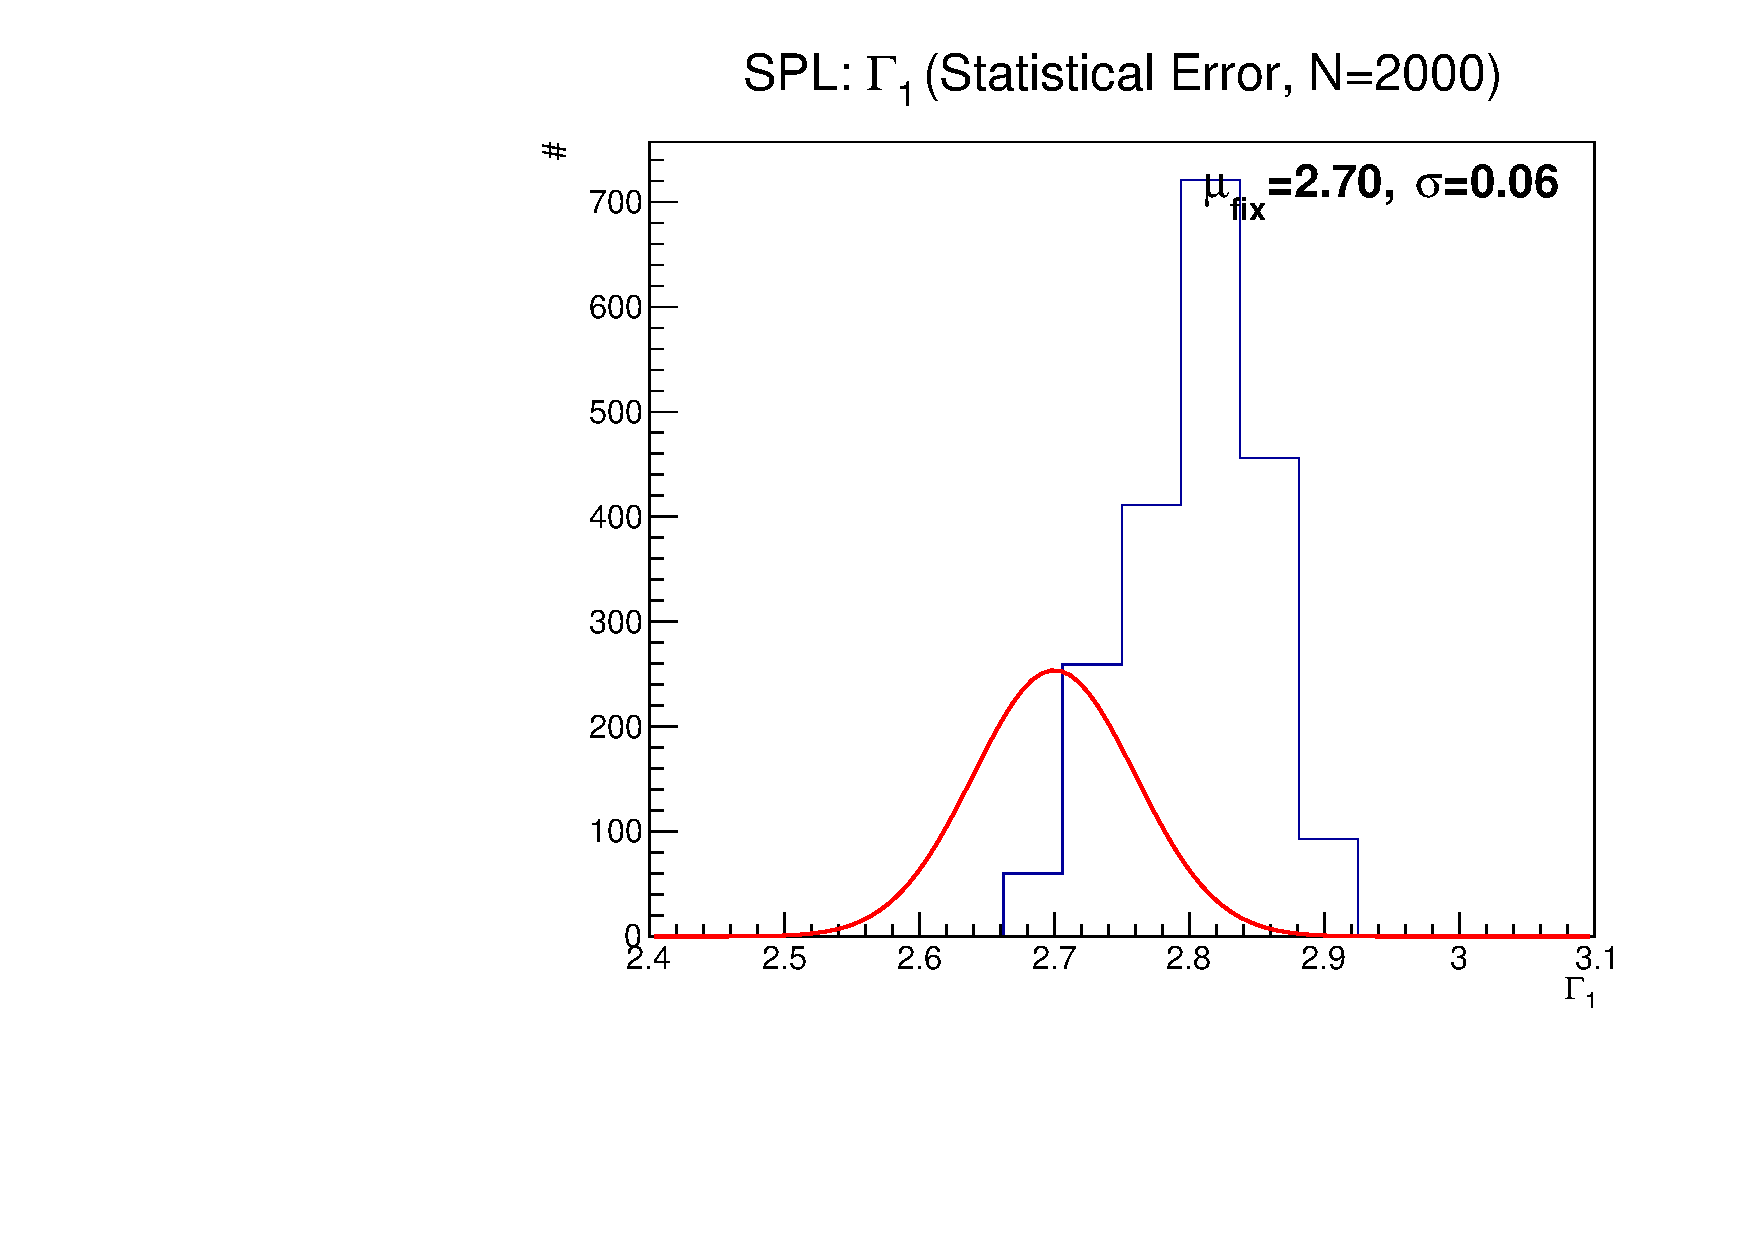
\includegraphics[width=0.48\textwidth]{appendix/montecarlo/figures/SPLwHe_gamma1_sys.pdf}
            }
        \hfill
         \subfloat[
            Total deviation
         ]{
            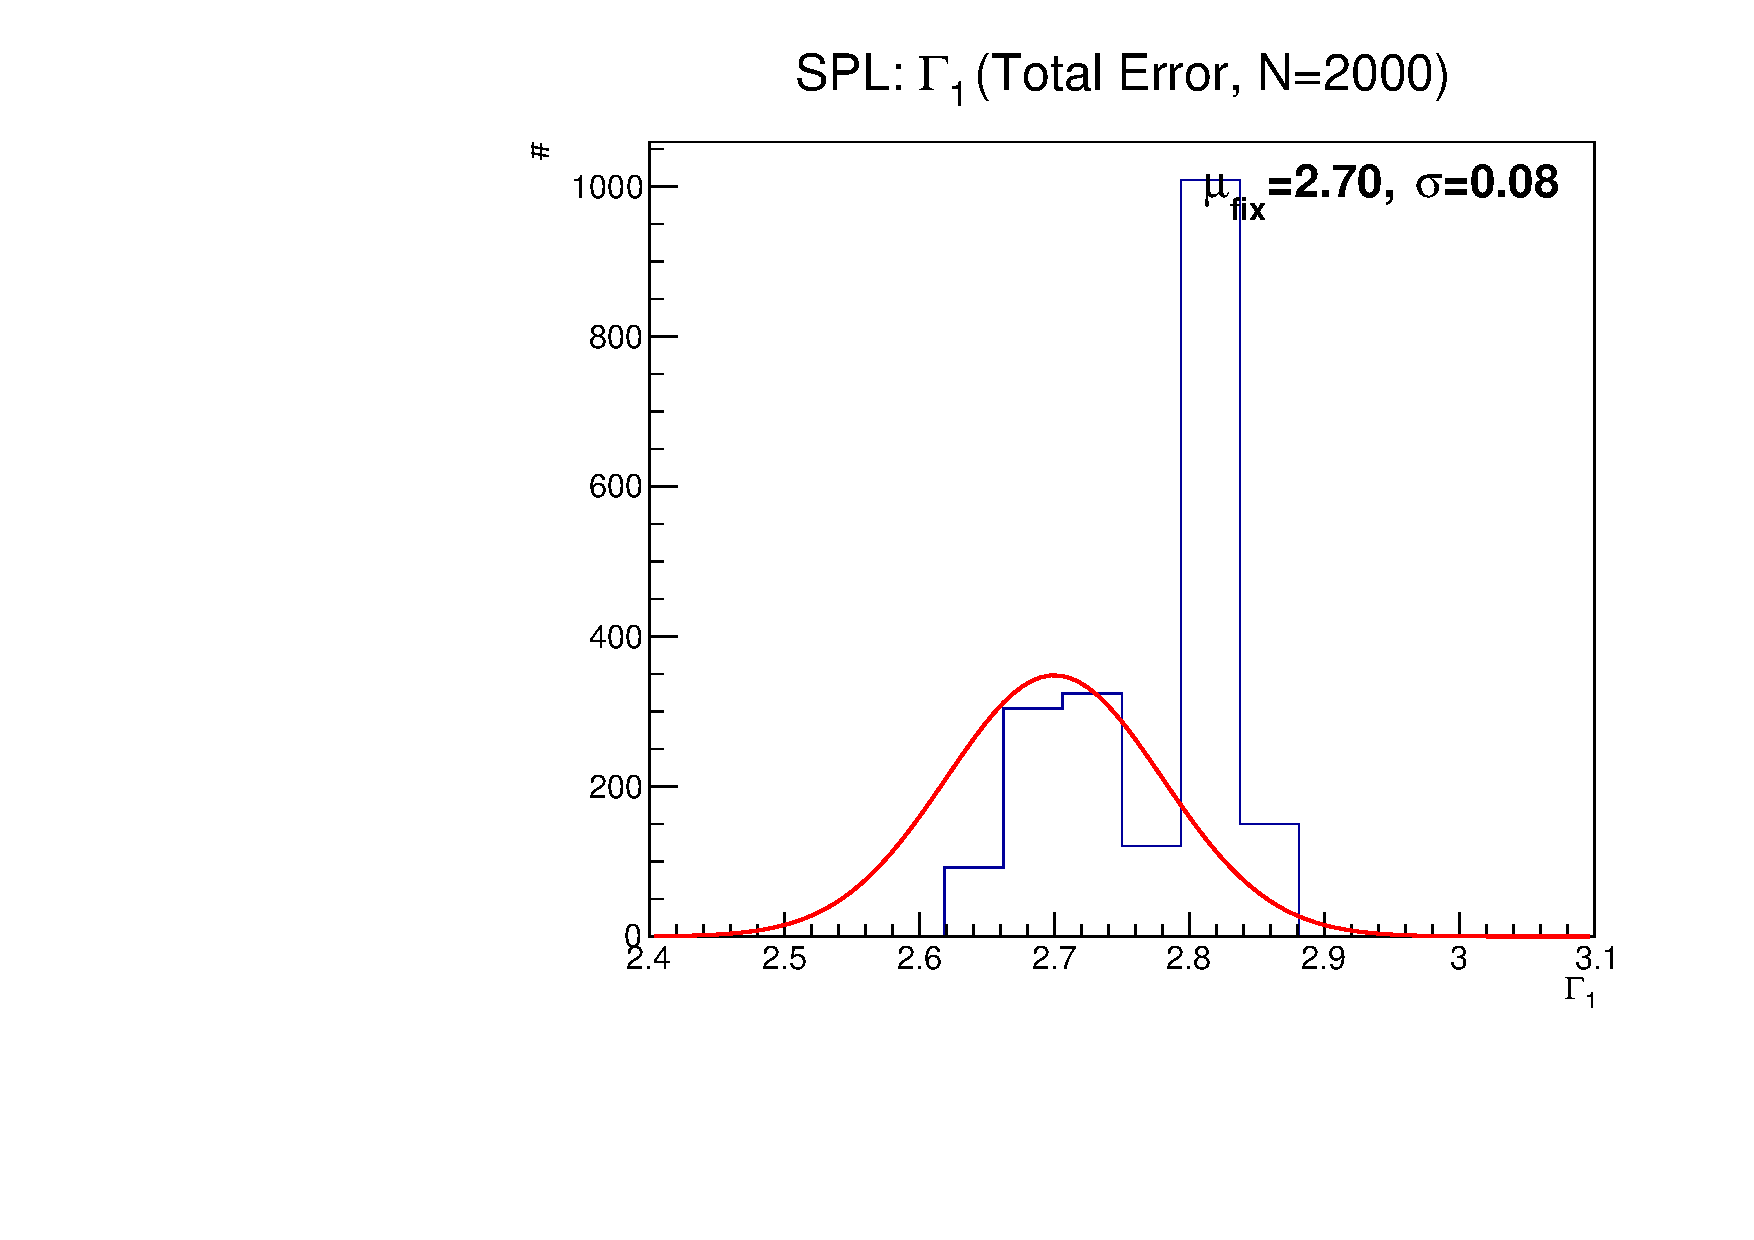
\includegraphics[width=0.48\textwidth]{appendix/montecarlo/figures/SPLwHe_gamma1_tot.pdf}
        }
        \caption{
            The distribution of the fitted results by
            % SPL model from the distortion.
            the SPL model of different simulated realizations of
            the Earth's $\gamma$-ray spectrum which is randomly
            distorted by the statistical (a) and total
            (b) uncertainties of the data.
        }
       \label{fig:monte_spl}
\end{figure}

Simulation process for statistical deviation is done by 
randomizing the photon count in each energy bin using
the poisson probability with the expected value being
the measured count.
Hence, each simulated realization of
the Earth's $\gamma$-ray spectrum
is distorted by statistical uncertainty of the measurement
and the best-fit parameters of the SPL and BPL models
of CR protons would reflect the underlying statistical uncertainty.
% rescaling the spectrum from the information of the arrival photon.
% The discrete probability of the events from a fixed amount
% of time could be modeled by using poisson distribution function.
% Hence, the photon spectrum in each energy bin will be rescaled
% by resampling photon numbers from a given amount of photon 
% from observations as the number of occurrences.
Results from statistical uncertainty analysis
using 2000 simulated realizations are shown
in Figure \ref{fig:monte_spl}a for the SPL model
and in Figure \ref{fig:monte_bpl_stat} for the BPL model.
% The results from the statistical simulation for SPL is shown in 
% Figure \ref{fig:monte_spl}a as well as Figure \ref{fig:monte_bpl_stat}
% demonstrates the deviation of BPL model.

\begin{figure}[h!]
    \centering
        \subfloat[First spectral index]{
            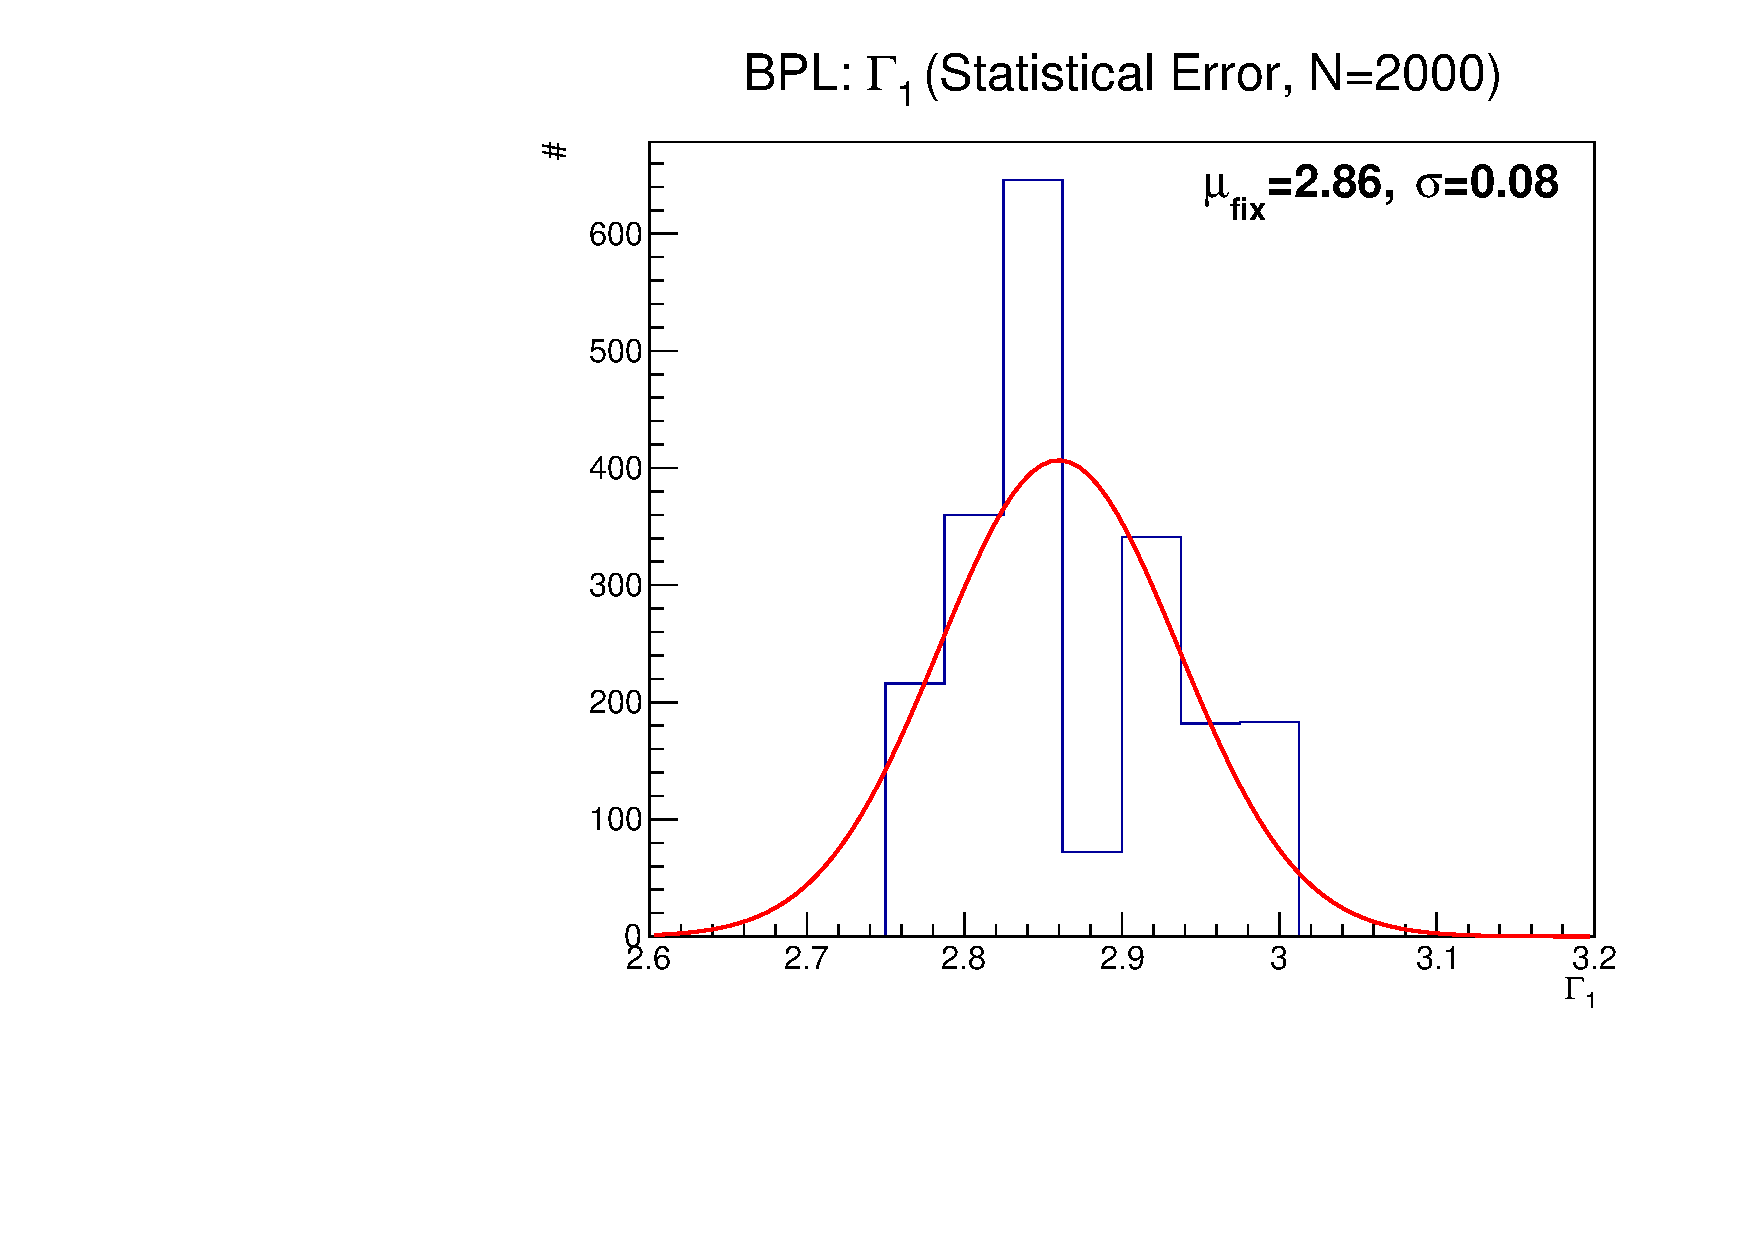
\includegraphics[width=0.33\textwidth]{appendix/montecarlo/figures/BPLwHe_gamma1_sys.pdf}
        }
        \subfloat[Second spectral index]{
            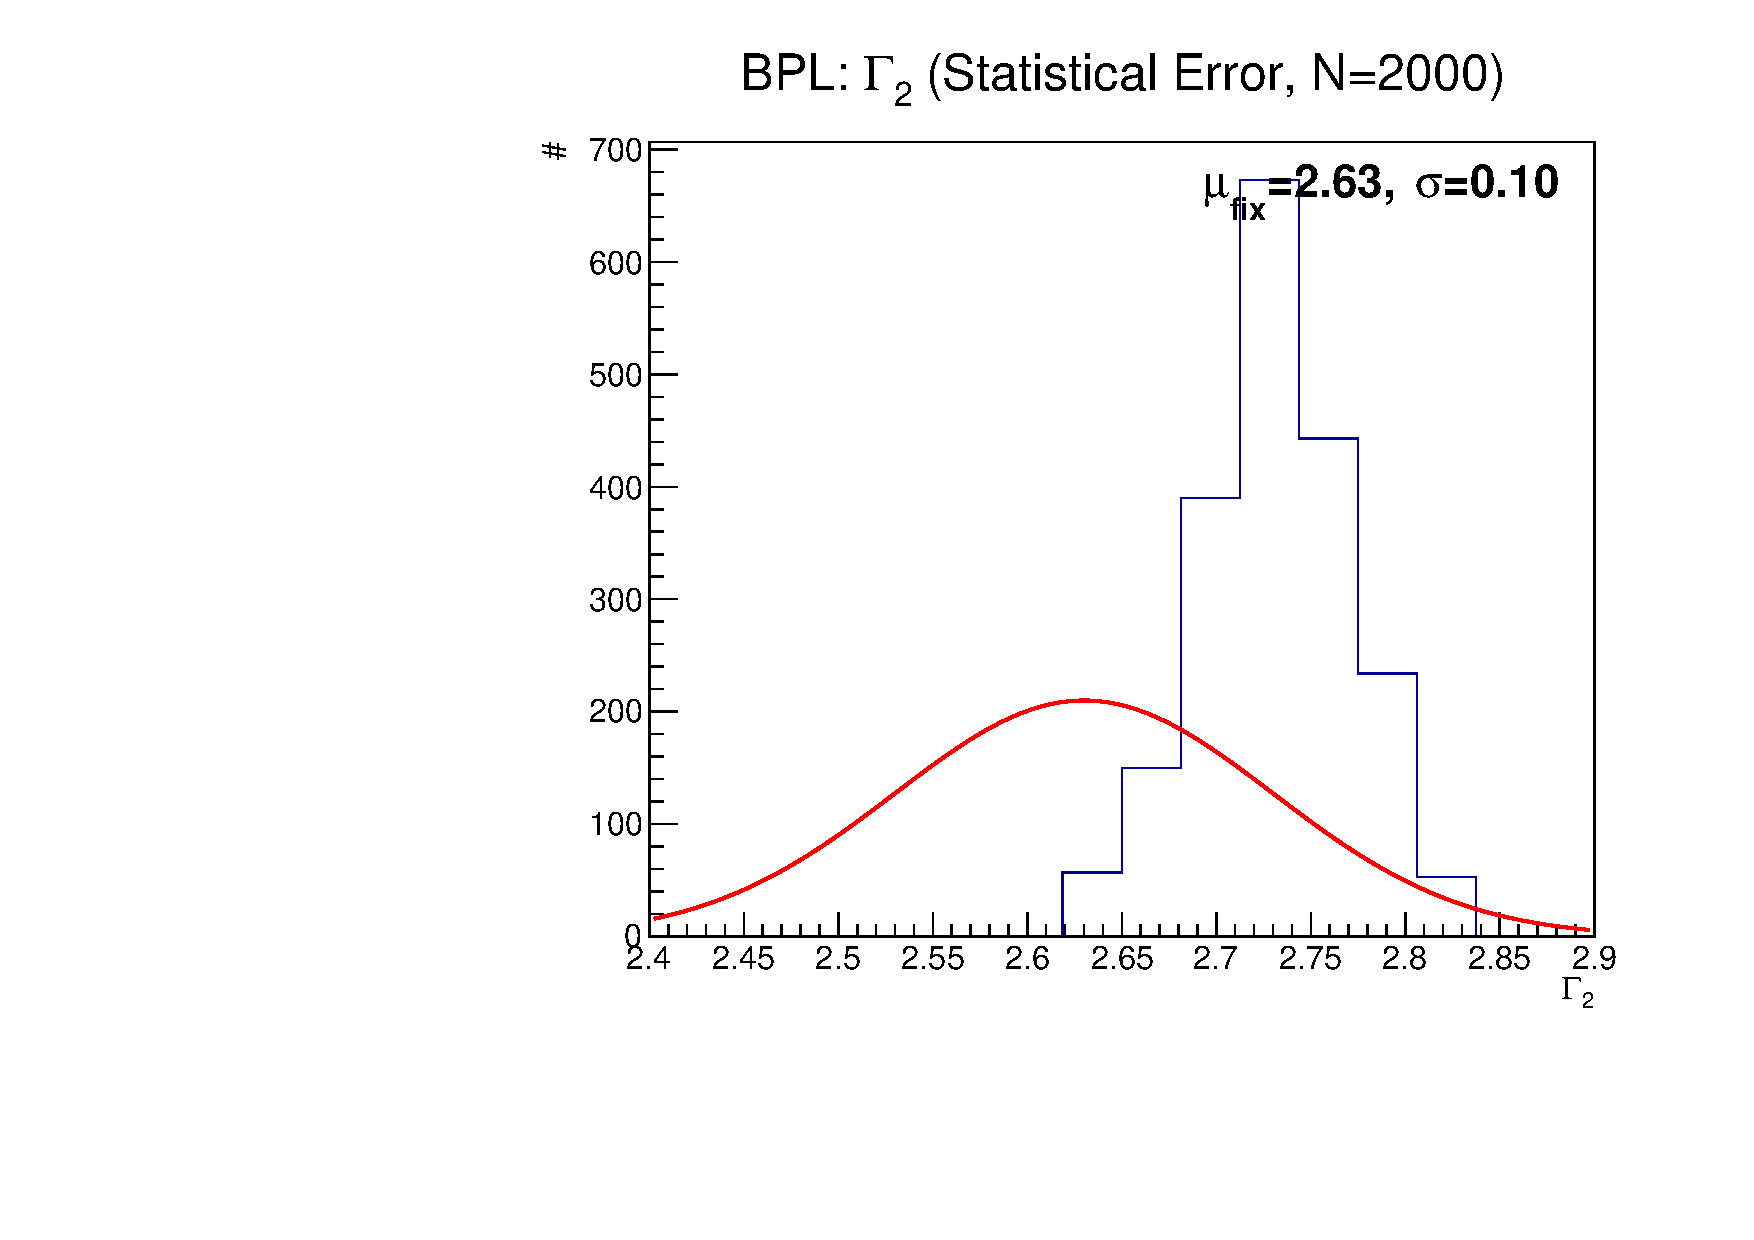
\includegraphics[width=0.33\textwidth]{appendix/montecarlo/figures/BPLwHe_gamma2_sys.pdf}
        }
        \subfloat[Breaking energy]{
            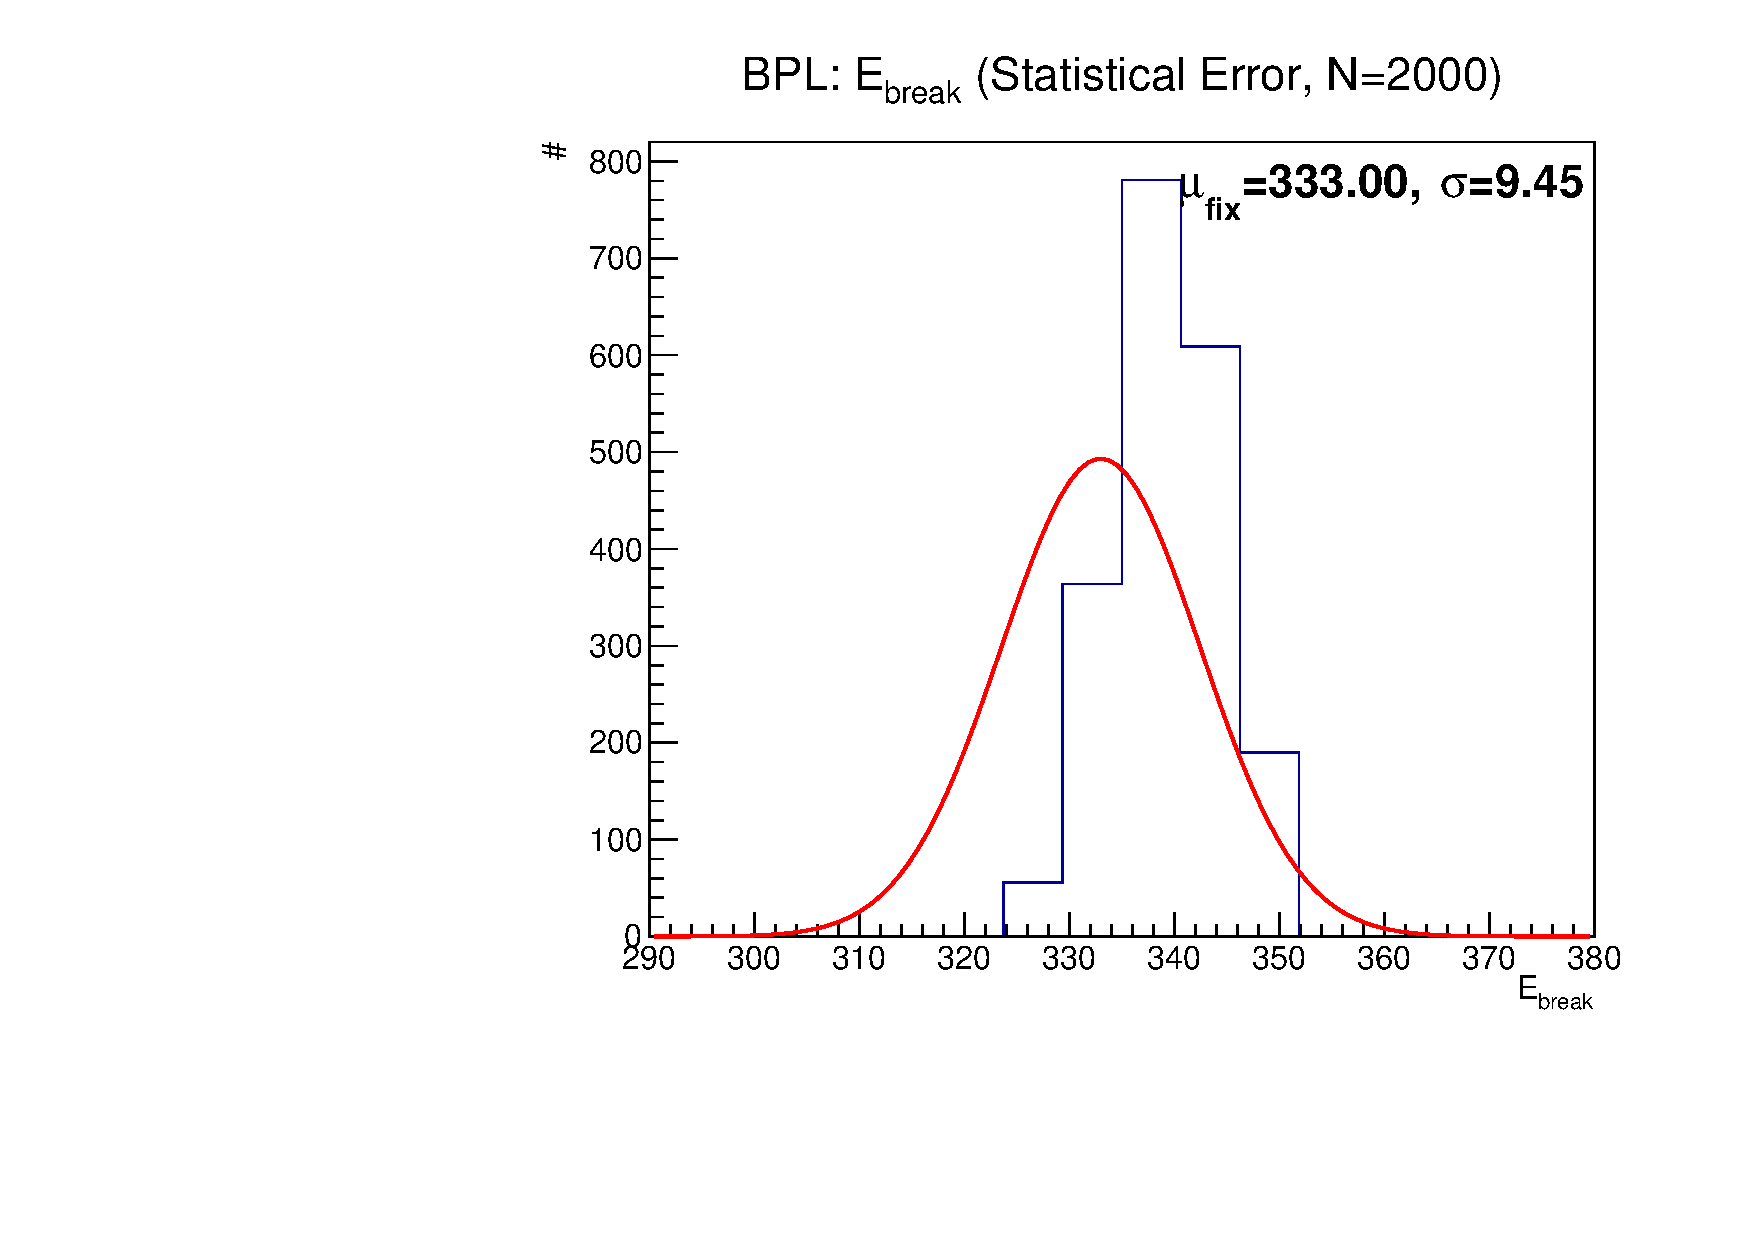
\includegraphics[width=0.33\textwidth]{appendix/montecarlo/figures/BPLwHe_e_break_sys.pdf}
        }        
        \caption{
            The distribution of the fitted results by the BPL model
            of different simulated realizations of the distorted Earth’s
            $\gamma$-ray spectrum by the
            statistical uncertainties of the data.
            The first spectral index ($\Gamma_1$),
            second spectral index ($\Gamma_2$) and 
            breaking energy ($E_\text{break}$) in GeV
            are shown in (a), (b) and (c) sequentially.
        }
       \label{fig:monte_bpl_stat}
\end{figure}



\begin{figure}[h!]
    \centering
        \subfloat[First spectral index]{
            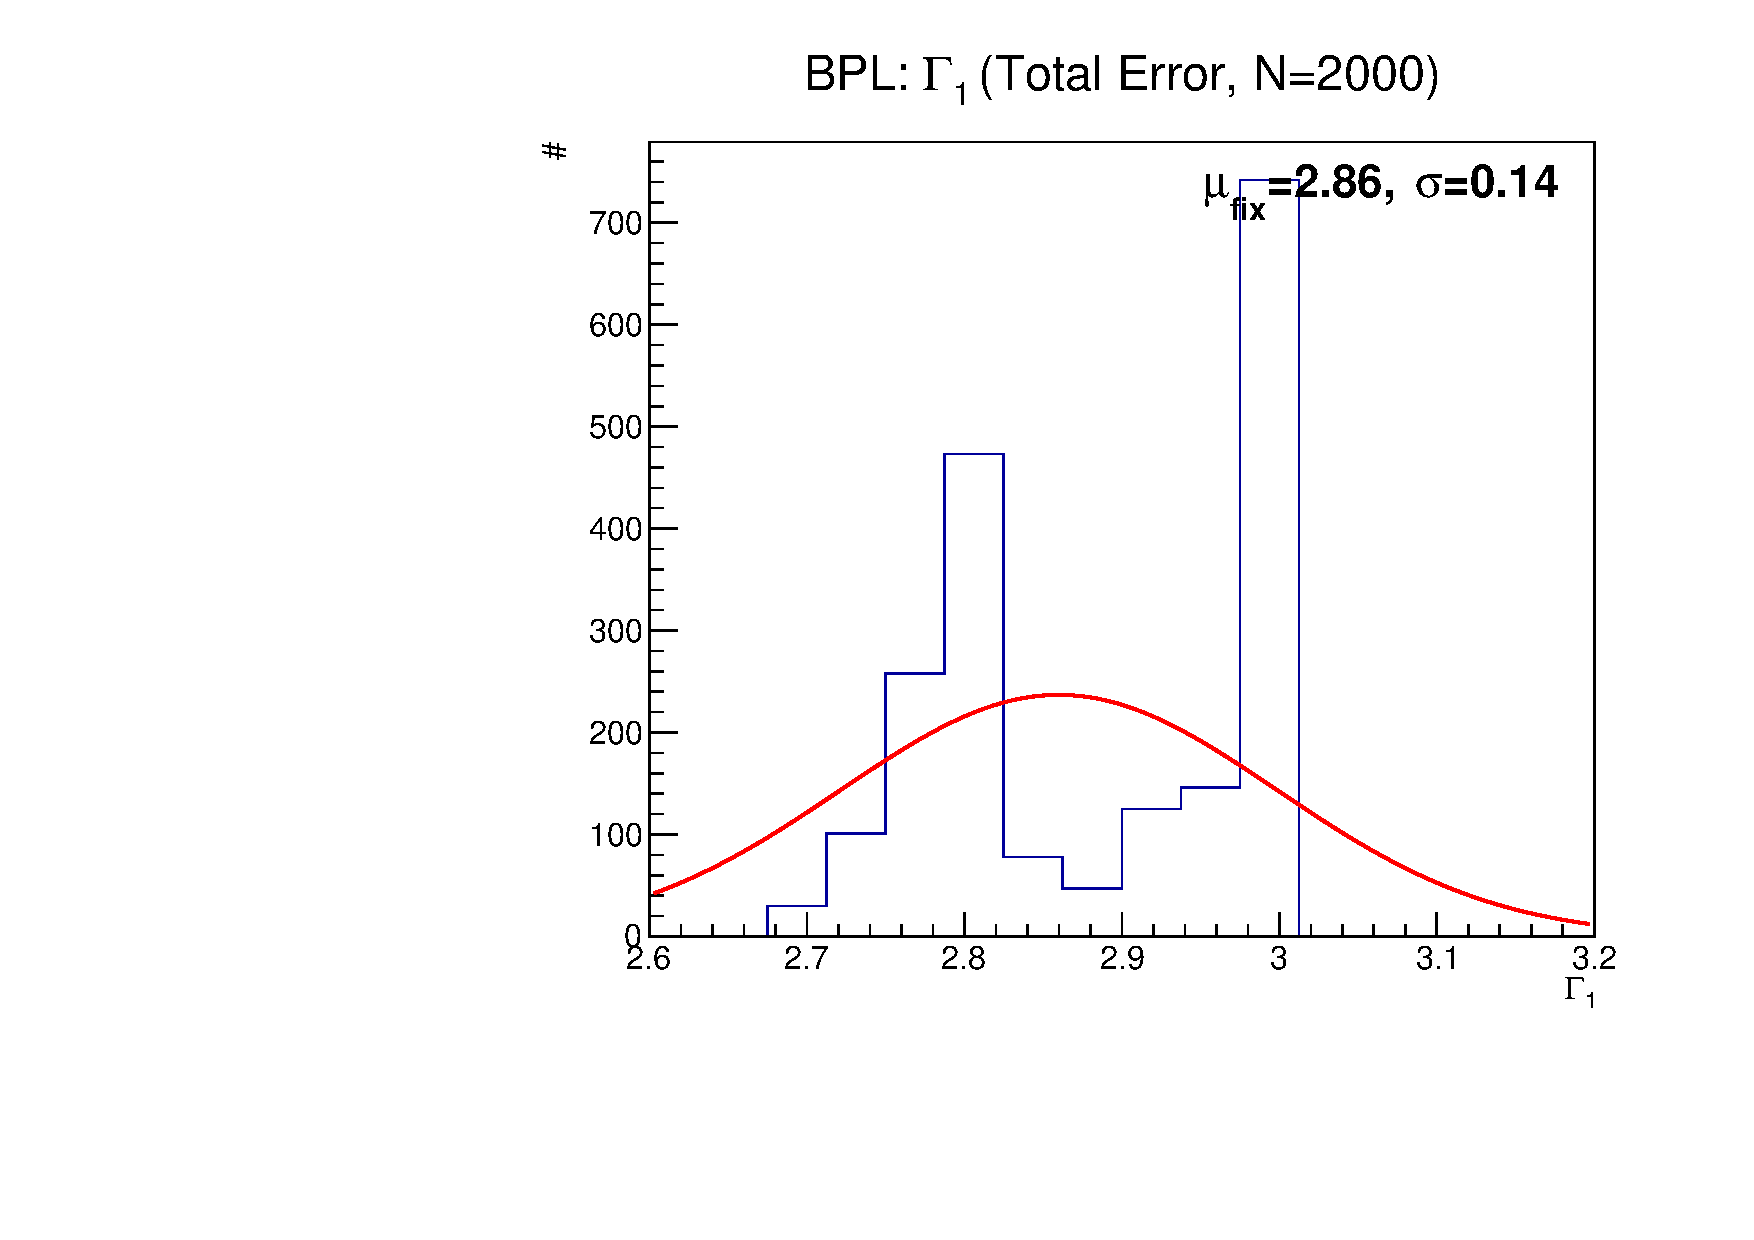
\includegraphics[width=0.33\textwidth]{appendix/montecarlo/figures/BPLwHe_gamma1_tot.pdf}
        }
        \subfloat[Second spectral index]{
            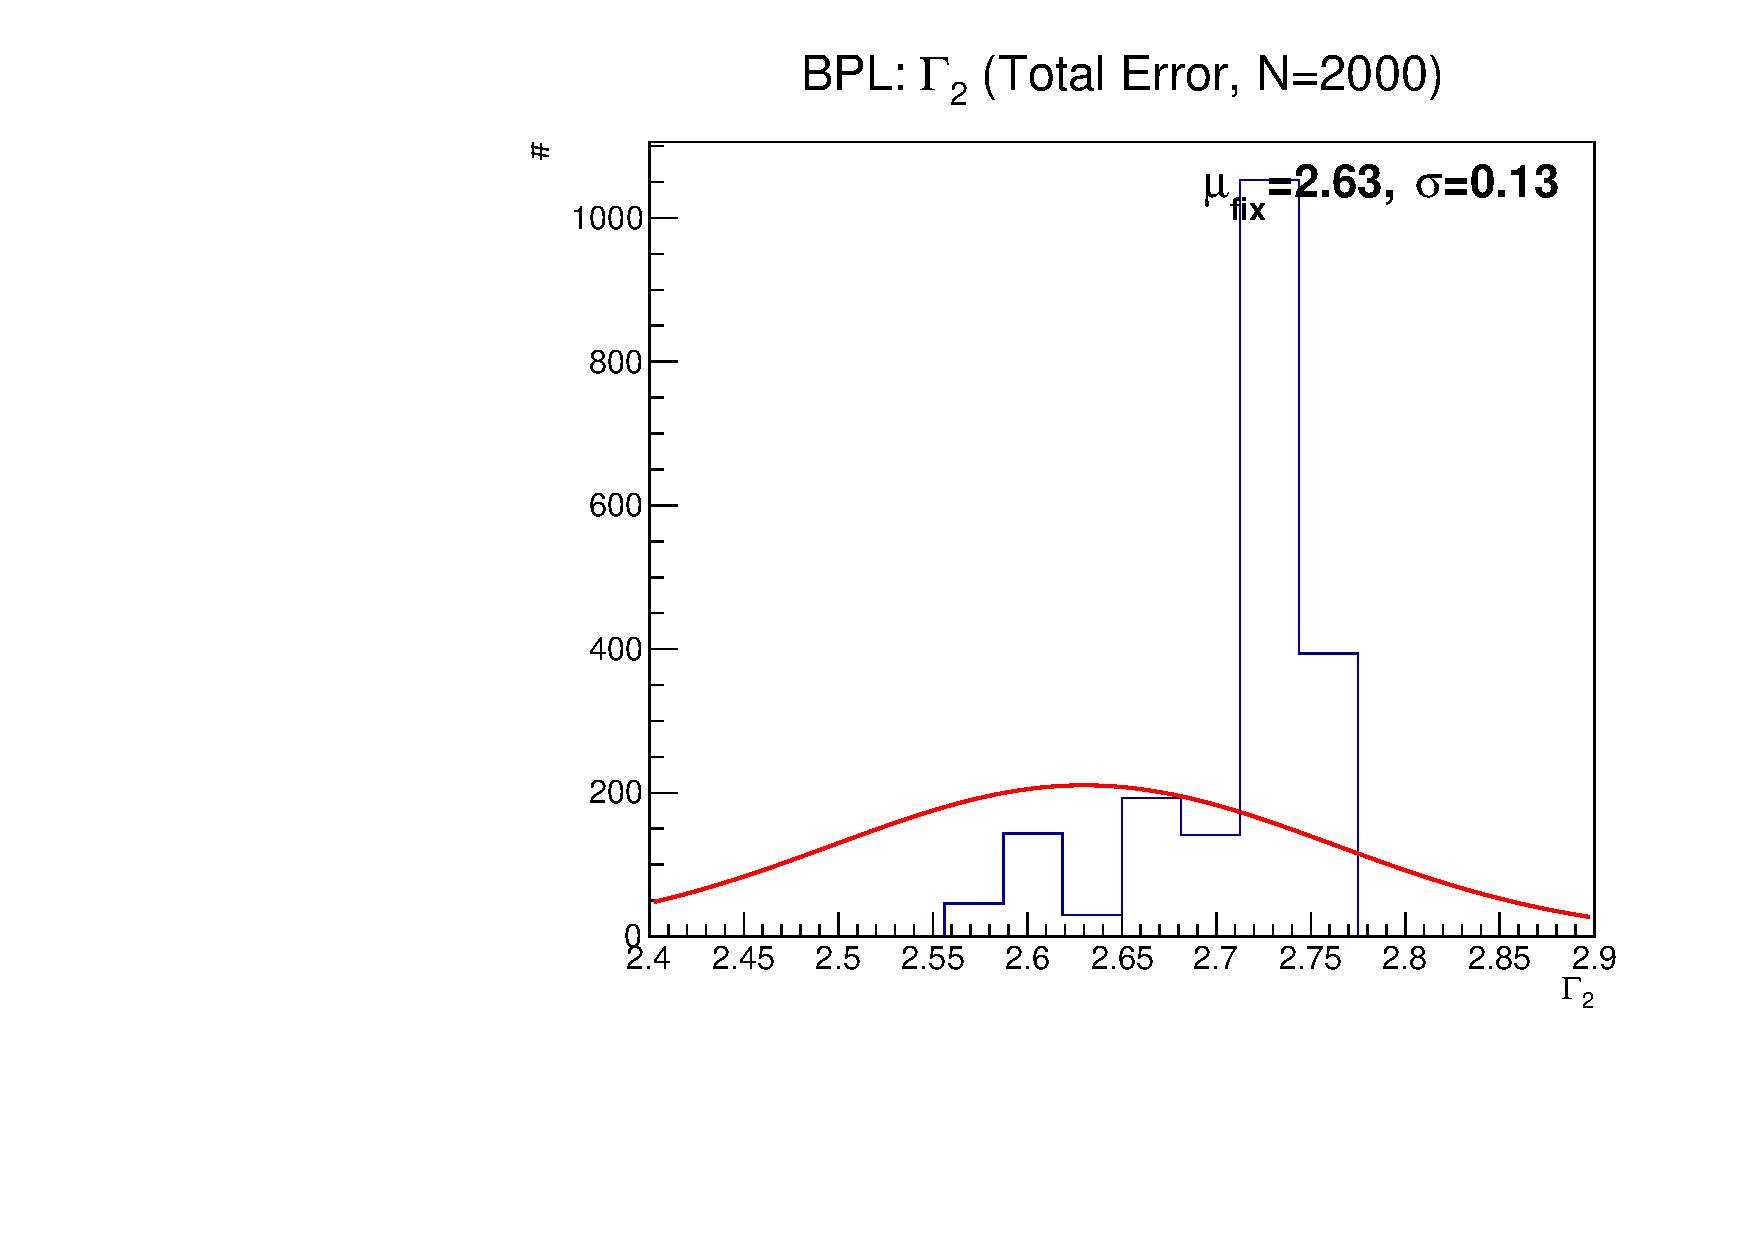
\includegraphics[width=0.33\textwidth]{appendix/montecarlo/figures/BPLwHe_gamma2_tot.pdf}
        }
        \subfloat[Breaking energy]{
            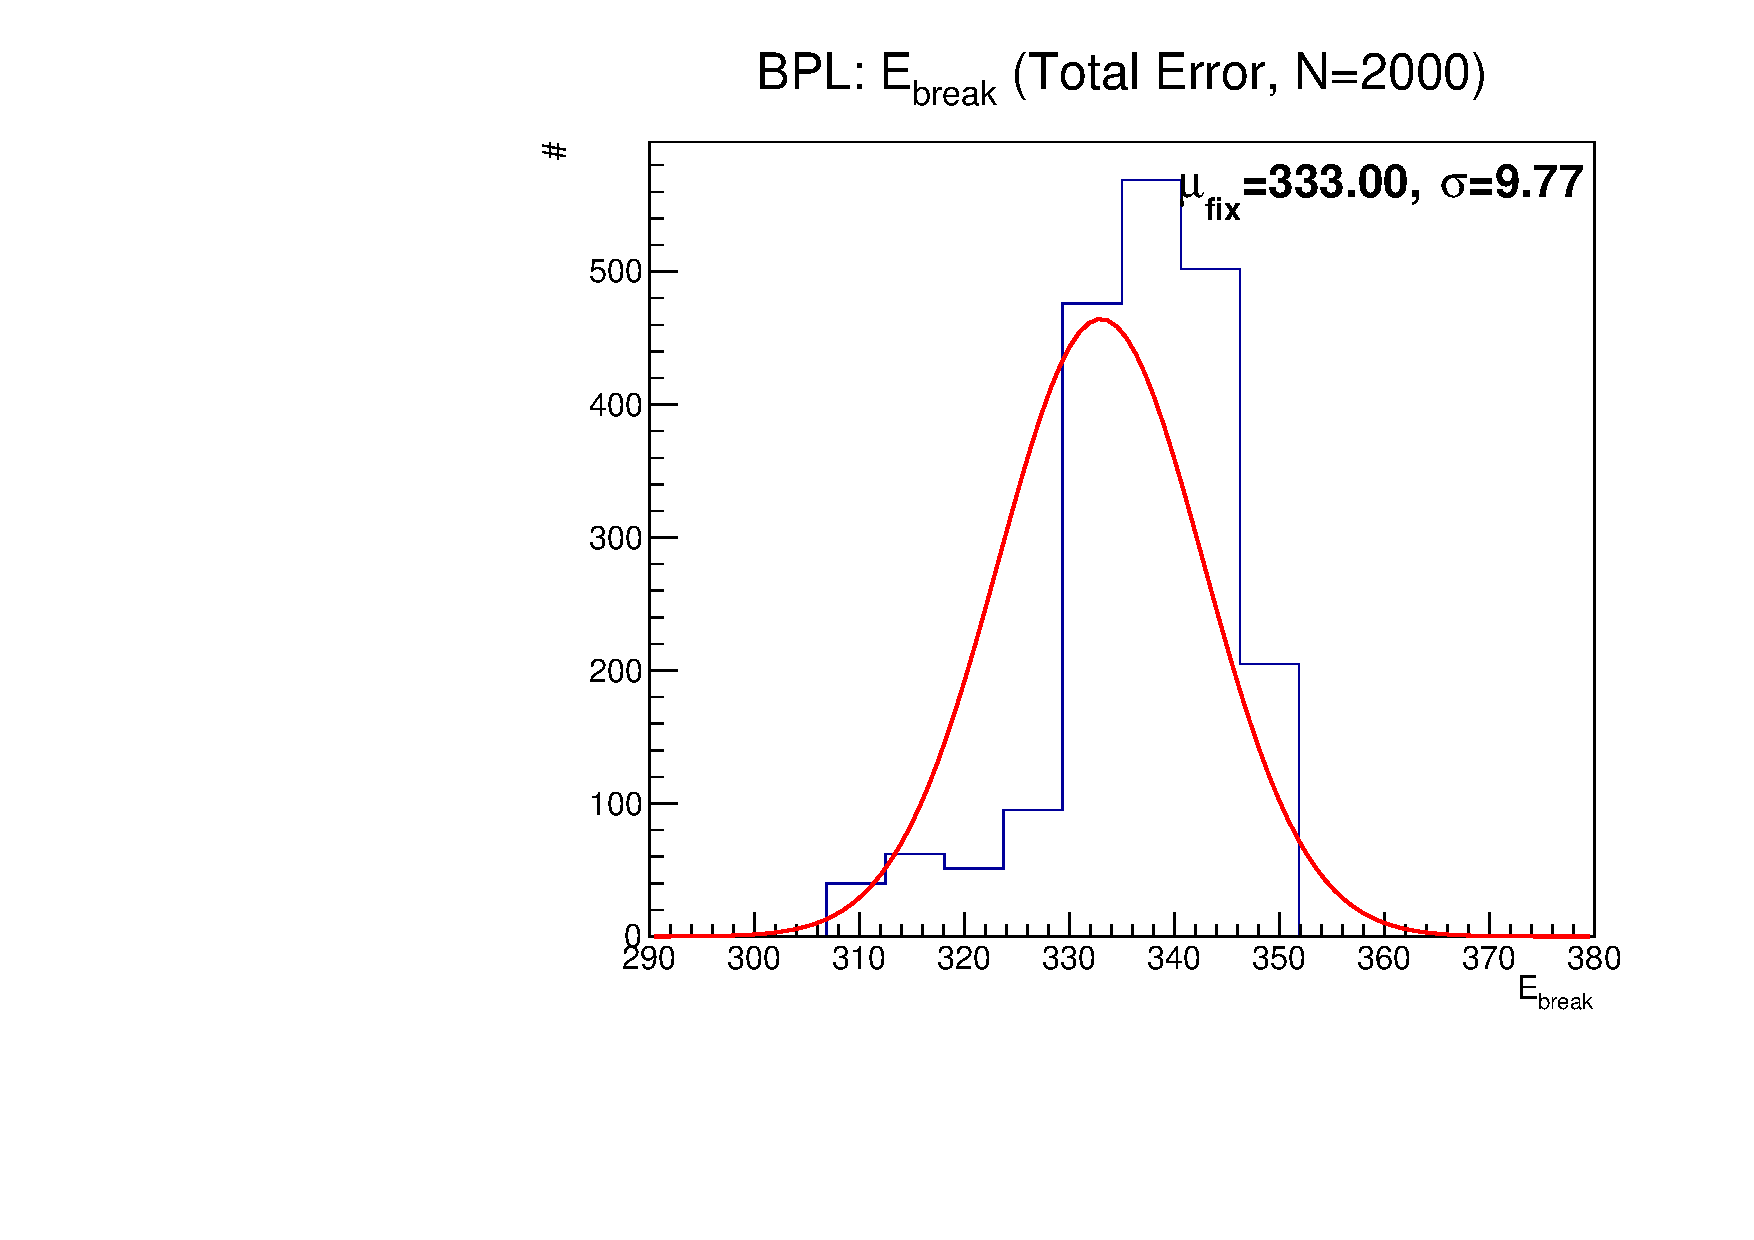
\includegraphics[width=0.33\textwidth]{appendix/montecarlo/figures/BPLwHe_e_break_tot.pdf}
        }        
        \caption{
            The distribution of the fitted results by the BPL model
            of different simulated realizations of the distorted Earth’s
            $\gamma$-ray spectrum by the
            statistical uncertainties and the systematical
            error from the instrument (total uncertainties).
            The first spectral index ($\Gamma_1$),
            second spectral index ($\Gamma_2$) and 
            breaking energy ($E_\text{break}$) in GeV
            are shown in (a), (b), and (c) sequentially.
        % Statistical and systematical (total) simulation of the BPL model
        }
       \label{fig:monte_bpl_tot}
\end{figure}


Total uncertainty estimation takes the systematic distortion
into
account by considering the uncertainty in the effective area of
% account. It is modeled as an uncertain from
the detector\footnote{\url{https://fermi.gsfc.nasa.gov/ssc/data/analysis/scitools/Aeff_Systematics.html}}.
First step for generating spectrum is exactly the same that for the
statistical error. The following step is to purturb the spectrum by
a distorted curve representing a possible realization of
the LAT effective area according to the estimated systematic uncertainty.
% the distorted curved.
The curve is computed by
sampling 3 values of the LAT effective area within
the uncertainty range (5\% at 10 GeV, 5\% at 100 GeV, and 15\% at 1 TeV)
assuming uniform probability and perform the cubic spline interpolation
through those 3 points. Distributions of the best-fit parameters
from 2000 simulated realizations of
the Earth's $\gamma$-ray spectrum distorted by the statistical
and systematic uncertainties for the SPL and BPL model are shown
in Figure \ref{fig:monte_spl}b and \ref{fig:monte_bpl_tot}, respectively. 
% sample three 
% different points in 3 energy decades (10 GeV, 100 GeV and 1 TeV).


% The results of the total error of SPL model is illustrated in
% Figure \ref{fig:monte_spl}b and the deviation of the BPL parameters
% is shown in Figure \ref{fig:monte_bpl_tot}.

